\chapter{Arhitektura i dizajn sustava}		
Arhitektura je podijeljena u tri pod sustava:

\begin{itemize}
	\item Web poslužitelj
	\item Web aplikacija
	\item Baza podataka	
\end{itemize}

\begin{figure}
	\centering
	
\includegraphics[width=0.5\textwidth]{Slike/ArhitekturaSustava}
	\caption{Arhitektura sustava}
	\label{fig:example}
\end{figure}

\textbf{Web preglednik} je program koji korisniku omogućuje pregled web-stranica, njenih multimedijskih sadržaja kao i slanje zahtjeva web poslužitelju. On ujedno i prevodi kod u kojem je napisana stranica u nešto raumljivo.
\newline
\indent\textbf{Web poslužitelj} kao posrednik između korisnika i aplikacije je osnova rada aplikacije. Komunikacija se ostvaruje HTTP  (engl. \textit{Hyper Text Transfer Protocol}) protokolom.
\newline
\indent\textbf{Web aplikacija} pomaže korisniku u obradi željenih zahtjeva. Web aplikacija po potrebi pristupa bazi podataka nakon čega korisniku vraća HTML dokument kojeg korisnik vidi u web pregledniku.
Programski jezik koji smo odabrali je Java zajedno sa Spring radnim okvirom i JavaScript. Odabrano razvojno okružje je Microsoft visual studio code i Intellij IDEA. Arhitektura sustava će se temeljiti na stilističkoj varijaciji arhitekture zasnovane na događajima (engl. \textit{event based architecture}) - MVC obrazcu.
\indent MVC (Model-View-Controller) obrazac je podržan od strane Spring radnog okvira i kao takav ima gotove predloške koji nam olakšavaju razvoj web aplikacije.
\newline
MVC obrazac omogućuje nezavisan razvoj pojedinih dijelova aplikacije što znatno olakšava ispitivanje kao i razvijanje i dodavanje novih svojstava u sustav.
\newline
Dijelovi MVC obrazca su:
\begin{itemize}
	\item Model - Centralna komponenta sustava predstavlja dinamičke strukture podataka koje su neovisne o ciljevima korisnika. Izravno upravlja podacima, logikom, i pravilima aplikacije, a isto tako prima ulazne podatke od kontrolera.
	\item View - Bilo kakav prikaz podataka, poput grafa. Moguci su različiti prikazi iste informacije poput grafičkog ili tabličnog prikaza podataka. 
	\item Controller - Prima ulaze i prilagođava ih za prosljeđivanje Modelu ili Viewu.
	Upravlja korisničkim zahtjevima i temeljem njih izvodi daljnju interakciju s ostalim elementima sustava.
\end{itemize}

				
		\section{Baza podataka}
			
		Za potrebe našeg sustava koristiti ćemo relacijsku bazu podataka koja svojom strukturom olakšava modeliranje stvarnog svijeta. Gradivna jedinka baze je relacija, odnosno tablica koja je definirana svojim imenom i skupom atributa. Zadaća baze podataka je brza i jednostavna pohrana, izmjena i dohvat podataka za daljnju obradu.
		Baza podataka ove aplikacije sastoji se od sljedećih entiteta: 
		
		\begin{itemize}
			\item Konferencija
			\item Korisnik
			\item Poster
			\item Pokrovitelj
			\item Pokrovitelj-Konferencije
			\item Fotografije
		\end{itemize}
		
			\subsection{Opis tablica}
				
				\noindent\textbf{Konferencija } Ovaj entitet sadržava sve važne informacije o stručnoj konferenciji. Sadrži atribute: Identifikator konferencije, ime konferencije, datum i vrijeme početka konferencije, datum i vrijeme završetka konferencije i mjesto održavanja konferencije. Ovaj entitet u vezi je \textit{One-to-Many} s entitetom Korisnik preko identifikatora konferencije, u vezi \textit{One-to-Many} s entitetom Poster preko identifikatora konferencije, u vezi \textit{One-to-Many} s entitetom Fotografije preko identifikatora konferencije i u vezi \textit{Many-to-Many} s entitetom Pokrovitelj preko identifikatora konferencije. 
				
				\begin{longtblr}[
					label=none,
					entry=none
					]{
						width = \textwidth,
						colspec={|X[6,l]|X[6, l]|X[20, l]|}, 
						rowhead = 1,
					} %definicija širine tablice, širine stupaca, poravnanje i broja redaka naslova tablice
					\hline \SetCell[c=3]{c}{\textbf{Konferencija}}	 \\ \hline[3pt]
					\SetCell{LightGreen}idKonferencije & INT	&  	jedinstveni brojčani identifikator konferencije  	\\ \hline
					ime Konferencije	& VARCHAR &   jedinstveno ime konferencije	\\ \hline 
					datumVrijeme Početka & DATETIME & datum i vrijeme početka konferencije  \\ \hline
					datumVrijeme Završetka & DATETIME & datum i vrijeme završetka konferencije \\ \hline
					mjesto	& VARCHAR & ime mjesta u kojem se održava konferencija \\ \hline 
				\end{longtblr}
				
				
				\noindent\textbf{Korisnik } Ovaj entitet sadržava sve važne informacije o korisniku aplikacije. Sadrži atribute: Korisničko ime, lozinku, ime, prezime, e-mail adresu korisnika, razinu ovlasti korisnika, identifikator konferencije na kojoj korisnik sudjeluje i identifikator postera za koji je korisnik glasao.  Ovaj entitet je u vezi \textit{Many-to-One} s entitetom Konferencija preko identifikatora konferencije, u vezi \textit{Many-to-One} s entitetom Poster preko identifikatora postera i u vezi \textit{One-to-One} s entitetom Poster preko korisničkog imena. 
				
				\begin{longtblr}[
					label=none,
					entry=none
					]{
						width = \textwidth,
						colspec={|X[6,l]|X[6, l]|X[20, l]|}, 
						rowhead = 1,
					} %definicija širine tablice, širine stupaca, poravnanje i broja redaka naslova tablice
					\hline \SetCell[c=3]{c}{\textbf{Korisnik}}	 \\ \hline[3pt]
					\SetCell{LightGreen}korisničko Ime & VARCHAR	&  jedinstveni identifikator korisnika 	\\ \hline
					lozinka	& VARCHAR & hash lozinka  	\\ \hline 
					ime & VARCHAR & ime korisnika  \\ \hline 
					prezime & VARCHAR	& prezime korisnika 		\\ \hline 
					email & VARCHAR	& e-mail adresa korisnika  		\\ \hline 
					razina ovlasti & INT &  razina ovlasti korisnika		\\ \hline 
					\SetCell{LightBlue} idKonferencije	& INT & jedinstveni identifikator konferencije na kojoj korisnik sudjeluje (konferencija.idKonferencije)  	\\ \hline 
					\SetCell{LightBlue} odabranPoster & INT & jedinstveni identifikator postera za koji je korisnik glasao (poster.id), ukoliko korisnik nije glasao vrijednost atributa je NULL \\ \hline
				\end{longtblr}
				
				\noindent \textbf{Poster } Ovaj entitet sadržava sve važne informacije o radu i/ili izlaganju koje je prikazano odgovarajućim posterom ili prezentacijom. Sadrži atribute: Identifikator postera, ime rada, broj glasova za poster, oznaku ima li prezentaciju, "prikaz" koji sadrži poster ili prezentaciju, identifikator konferencije na kojoj se rad izlaže i identifikator korisnika koji je autor rada. Ovaj entitet je u vezi \textit{Many-to-One} s entitetom Konferencija preko identifikatora konferencije, u vezi \textit{One-to-Many} s entitetom Korisnik preko identifikatora postera i u vezi \textit{One-to-One} s entitetom Korisnik preko korisničkog imena. 
				
				
				\begin{longtblr}[
					label=none,
					entry=none
					]{
						width = \textwidth,
						colspec={|X[6,l]|X[6, l]|X[20, l]|}, 
						rowhead = 1,
					} %definicija širine tablice, širine stupaca, poravnanje i broja redaka naslova tablice
					\hline \SetCell[c=3]{c}{\textbf{Poster}}	 \\ \hline[3pt]
					\SetCell{LightGreen}id & INT	&  jedinstveni brojčani identifikator	\\ \hline
					brojGlasova	& INT & broj glasova za poster  	\\ \hline 
					imeRada & VARCHAR & ime rada kojeg poster prikazuje \\ \hline
					prezentacija & BOOLEAN & oznaka ima li prezentaciju  \\ \hline 
					prikaz & LONGBLOB	& slika postera ukoliko je vrijednost atributa prezentacija jednaka FALSE, inače je priložena prezentacija u PDF obliku 		\\ \hline 
					\SetCell{LightBlue} idKonferencije	& INT & jedinstveni brojčani identifikator konferencije kojoj poster pripada (konferencija.idKonferencije)  	\\ \hline 
					\SetCell{LightBlue} autor	& VARCHAR & jedinstveni identifikator autora rada kojeg poster prikazuje (korisnik.korisničkoIme)  	\\ \hline 
				\end{longtblr}
				
				
				\noindent \textbf{Pokrovitelj } Ovaj entitet sadržava sve važne informacije o pokrovitelju. Sadrži atribute: Identifikator pokrovitelja, ime pokrovitelja i promotivne materijale. Ovaj entitet je u vezi \textit{Many-to-Many} s entitetom Konferencija.
				
				
				\begin{longtblr}[
					label=none,
					entry=none
					]{
						width = \textwidth,
						colspec={|X[6,l]|X[6, l]|X[20, l]|}, 
						rowhead = 1,
					} %definicija širine tablice, širine stupaca, poravnanje i broja redaka naslova tablice
					\hline \SetCell[c=3]{c}{\textbf{Pokrovitelj}}	 \\ \hline[3pt]
					\SetCell{LightGreen}idPokrovitelja & INT & jedinstveni brojčani identifikator pokrovitelja  	\\ \hline
					ime
					Pokrovitelja	& VARCHAR & jedinstveno ime pokrovitelja   	\\ \hline 
					promo & LONGBLOB & promotivni materijal; slika loga pokrovitelja   \\ \hline 
				\end{longtblr}
				
				
				\noindent \textbf{Pokrovitelj-Konferencije } Ovaj entitet sadržava sve informacije o odnosu konferencije i pokrovitelja odnosno kojoj konferenciji pokrovitelj pripada.
				
				
				\begin{longtblr}[
					label=none,
					entry=none
					]{
						width = \textwidth,
						colspec={|X[6,l]|X[6, l]|X[20, l]|}, 
						rowhead = 1,
					} %definicija širine tablice, širine stupaca, poravnanje i broja redaka naslova tablice
					\hline \SetCell[c=3]{c}{\textbf{Pokrovitelj-Konferencije}}	 \\ \hline[3pt]
					\SetCell{LightBlue} idPokrovitelja	& INT & jedinstveni brojčani identifikator pokrovitelja (pokrovitelj.idPokrovitelja)     	\\ \hline
					\SetCell{LightBlue}idKonferencije	& INT & jedinstveni brojčani identifikator konferencije (konferencija.idKonferencije)  	\\ \hline 

				\end{longtblr}
				
				
				\noindent \textbf{Fotografija } Ovaj entitet sadržava sve informacije o fotografijama s konferencije. Sadrži atribute: Identifikator fotografije, sliku fotografije i identifikator konferencije koja je fotografirana. Ovaj entitet u vezi je \textit{Many-to-One} s entitetom Konferencija. 
				
				
				\begin{longtblr}[
					label=none,
					entry=none
					]{
						width = \textwidth,
						colspec={|X[6,l]|X[6, l]|X[20, l]|}, 
						rowhead = 1,
					} %definicija širine tablice, širine stupaca, poravnanje i broja redaka naslova tablice
					\hline \SetCell[c=3]{c}{\textbf{Fotografije}}	 \\ \hline[3pt]
					\SetCell{LightGreen}id & INT & jedinstveni brojčani identifikator fotografije   	\\ \hline
					slika	& LONGBLOB &  fotografija s konferencije	\\ \hline 
					\SetCell{LightBlue} idKonferencije	& INT & jedinstveni brojčani identifikator konferencije (konferencija.idKonferencija)  	\\ \hline 
				\end{longtblr}
			
			\subsection{Dijagram baze podataka}
				
					\begin{figure} [h]
						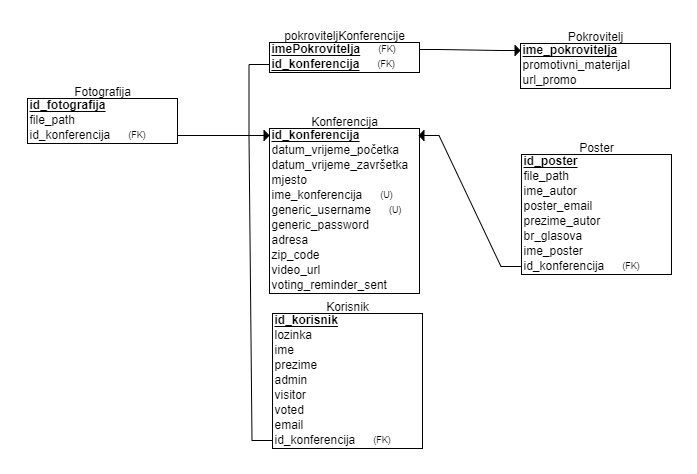
\includegraphics[width=\linewidth]{Slike/ERDijagram}
						\caption{E-R dijagram baze podataka}
					\end{figure}
			
			\eject
			
			
		\section{Dijagram razreda}
			
			Na slikama 4.2 i 4.3 su prikazani  razredi koji pripadaju \textit{backend} dijelu MVC arhitekture. Razredi prikazani na slici 4.2 nasljeđuju Controller razred. Metode implementirane u tim razredima manipuliraju s DTO (\textit{Data transfer object}), a oni su dohvaćeni pomoću metoda implementiranih u Model razredima. Metode implementiranih u Model razredima. Metode implenetirane u Controller razredima vraćaju JSON datoteke s html status kodom.
			
			Zbog lakše organizacije, razredi su podijeljeni logički po pravu pristupa metodama određenih aktora, kako bi se smanjila prenapučenost unutar dijagrama, prikazane su samo ovisnosti između razreda koji pripadaju istom dijelu dijagrama. Iz naziva i tipova atributa u razredima može se zaključiti vrsta ovisnosti među različitim razredima. 
			
			\begin{figure} [h]
				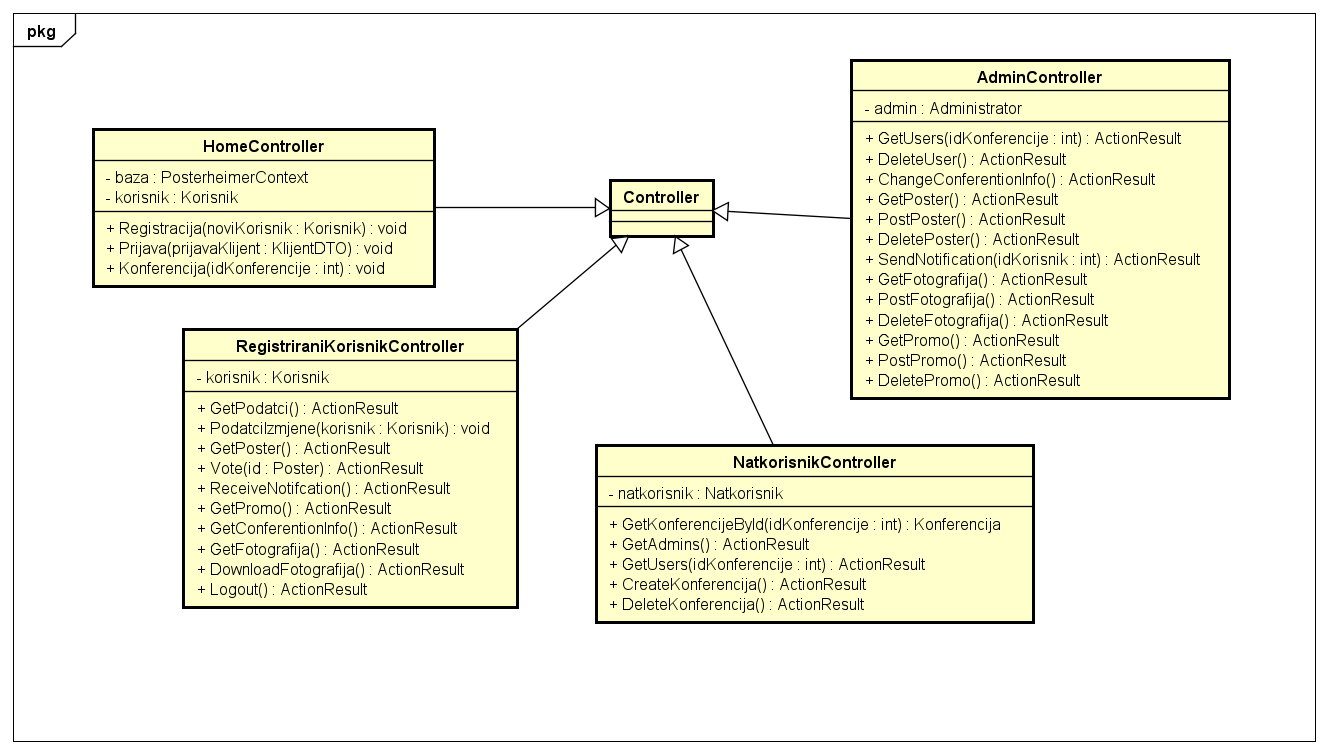
\includegraphics[width=\linewidth]{Slike/ClassDiagramControllers}
				\caption{Dijagram razreda - dio Controllers}
			\end{figure}
			
			Model razredi preslikavaju strukturu baze podataka u aplikaciji. Implementirane metode direktno komuniciraju s bazom podataka te vraćaju tražene podatke. Razred Korisnik predstavlja neregistriranog korisnika koji se može registrirati u sustav unoseći osnove informacije. Razred RegistriraniKorisnik predstavlja korisnika koji je registriran u sustav i koji može koristiti njegove osnove funkcionalnosti. Razred Administratora predstavlja administratora sustava koji ima najveće ovlasti. Razred Natkorisnika predstavlja natkorisnika koji ima mogućnost upravljanja konferencijama i postavljanje administratora. Razred Konferencija predstavlja skup podataka koji su potrebni za registraciju konferencije i koji se prikazuju korisnicima. Razred Poster predstavlja skup podataka koji su potrebni za dodavanje postera i koji se prikazuju korisnicima. Razred Fotografije predstavlja skup podataka vezan uz pojedinačnu fotografiju konferencije. Razred Pokrovitelj predstavlja pokrovitelja konferencije. 
			
			\begin{figure} [h]
				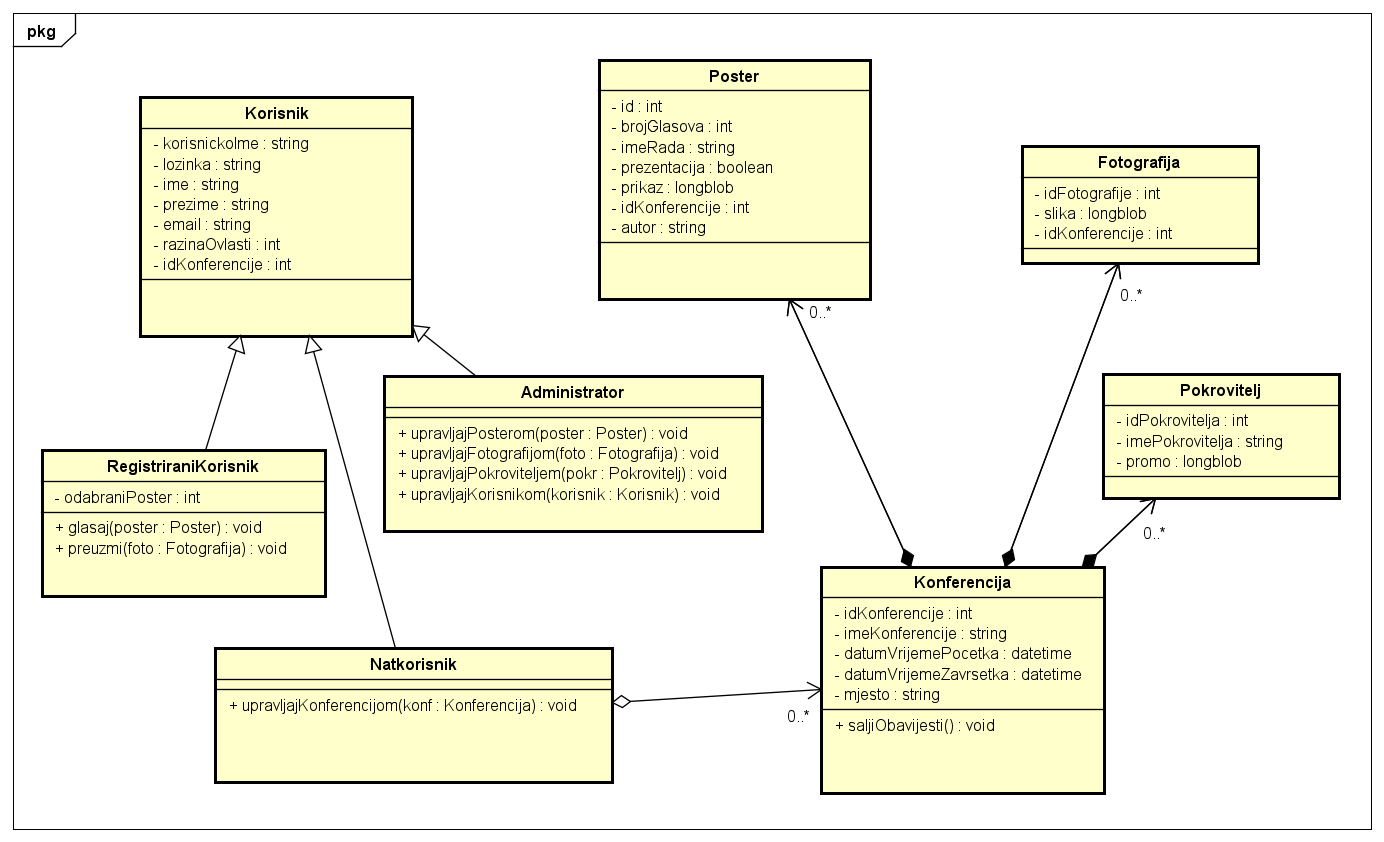
\includegraphics[width=\linewidth]{Slike/ClassDiagram}
				\caption{Dijagram razreda - dio Models}
			\end{figure}
			
			\textbf{\textit{dio 2. revizije}}\\			
			
			\textit{Prilikom druge predaje projekta dijagram razreda i opisi moraju odgovarati stvarnom stanju implementacije}
			
			
			
			\eject
		
		\section{Dijagram stanja}
			
			
			\textbf{\textit{dio 2. revizije}}\\
			
			\textit{Potrebno je priložiti dijagram stanja i opisati ga. Dovoljan je jedan dijagram stanja koji prikazuje \textbf{značajan dio funkcionalnosti} sustava. Na primjer, stanja korisničkog sučelja i tijek korištenja neke ključne funkcionalnosti jesu značajan dio sustava, a registracija i prijava nisu. }
			
			
			\eject 
		
		\section{Dijagram aktivnosti}
			
			\textbf{\textit{dio 2. revizije}}\\
			
			 \textit{Potrebno je priložiti dijagram aktivnosti s pripadajućim opisom. Dijagram aktivnosti treba prikazivati značajan dio sustava.}
			
			\eject
		\section{Dijagram komponenti}
		
			\textbf{\textit{dio 2. revizije}}\\
		
			 \textit{Potrebno je priložiti dijagram komponenti s pripadajućim opisom. Dijagram komponenti treba prikazivati strukturu cijele aplikacije.}